\subsection{App per imparare}
Inizio questo capitolo con le app che più utilizzo per informarmi.

\begin{itemize}
\item Feedly: Ci sono tanti siti che pubblicano news su cui vorrei rimanere aggiornato, ma andare periodicamente su
ognuno di questi siti per vedere gli aggiornamenti può diventare un lavoro impegnativo. Feedly ci viene in contro in
quanto ci permette di aggiungere in un unico posto tutte le nostre fonte di informazioni e vedere ogni nuovo articolo
che viene pubblicato. Tra i miei siti preferiti troviamo: Focus, National Geographic, TedVice, Wired. Oltre ai siti si
possono aggiungere podcast, come Daily cogito e Psinel o canali Youtube come quello di Just Mick, Luca Mazzucchelli e
Wesa channell.
\item Google Play Books: Per quanto riguarda la lettura di libri apprezzo Google Play Books, perché oltre ad essere
forse il più grosso store, l'app per smartphone ha anche la funzione di sintesi vocale. Questa
funzione permette di farsi leggere il libro da una voce artificiale. Questa lettura, essendo fatta da un software e non
da una persona in carne ed ossa, non risulta certamente espressiva, ma nemmeno così robotica come ci si potrebbe
immaginare. Dopo poco ci si abitua e l'esperienza risulta più che fruibile. Ho iniziato ad
apprezzare questa funzione durante i miei viaggi in macchina di circa un ora per raggiungere il luogo di lavoro.
Sentivo che quel tempo poteva essere impiegato in modo migliore e così ho introdotto la lettura.
\item Ereader Prestigio: Se abbiamo dei documenti in Pdf, al momento della stesura di queste righe, Google Play Books
non permette la sintesi vocale. Per questo possiamo utilizzare eReader. Entrambe le applicazioni consentono di
impostare la sintesi vocale a velocità diverse. Possiamo impostarla a 1,25x, 1.5x, 1,75x o 2x, con
quest'ultima opzione significa che il lettore parlerà due volte più veloce del normale.
\raggedright\url{https://play.google.com/store/apps/details?id=com.prestigio.ereader} 
\item Youtube: Fin ora abbiamo visto come fruire di contenuti testuali, ma da casa Google troviamo
quelle che secondo me sono le app più ricche di contenuti per quanto riguardano podcast e video.
\end{itemize}

\needspace{4cm}
\subsection{Sokushinbutsu}

\begin{wrapfigure}{i}{9cm}
  \centering
  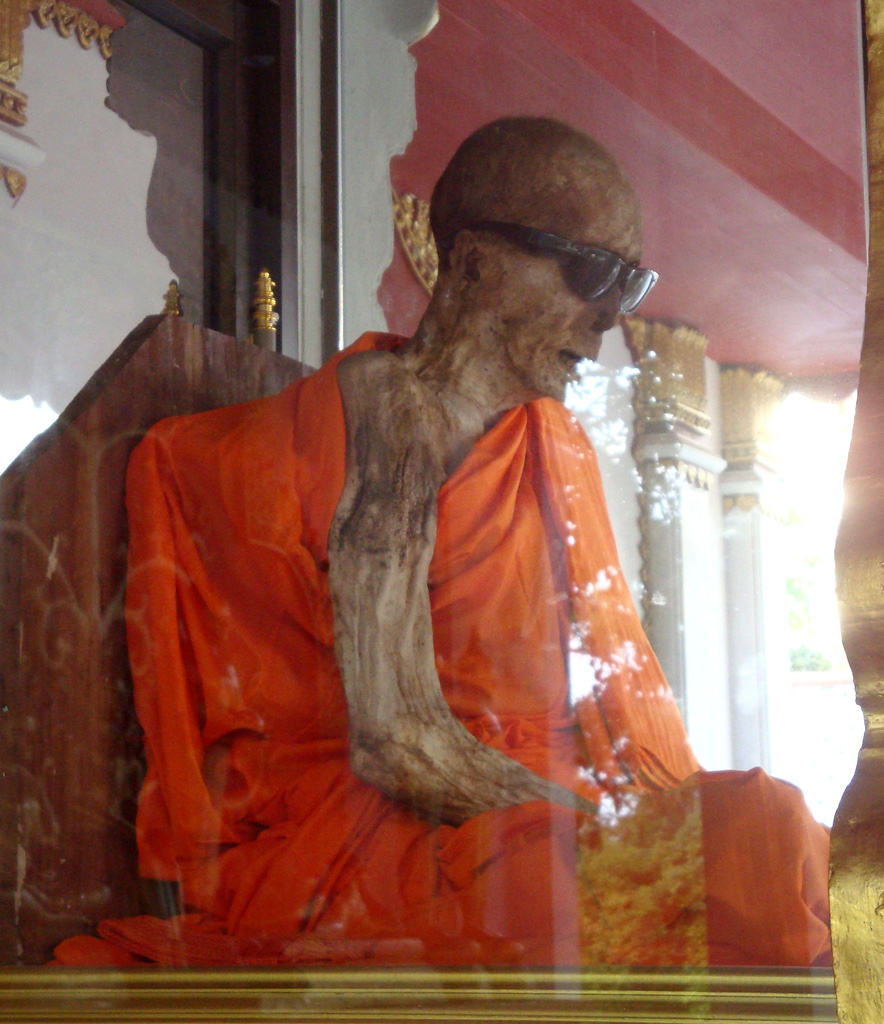
\includegraphics[width=0.95\linewidth]{images/Libro-img042.jpg}
  \begin{minipage}{\linewidth}
    \caption{Credits: Di Per Meistrup, CC BY-SA 3.0, \raggedright\url{https://commons.wikimedia.org/w/index.php?curid=19168593}}
  \end{minipage}
\end{wrapfigure}

Questa cosa mi ha letteralmente scioccato, si tratta di un rituale religioso buddhista, praticato dai monaci giapponesi
i quali, attraverso un lungo processo che terminava con la morte riuscivano ad automummificarsi. 

Questo processo, che si svolge da vivi, si divide in tre fasi, ognuna della durata di mille giorni dove progressivamente
ci si priva del cibo e si incrementa la meditazione e l'esercizio fisico.

Nella prima fase, il monaco si reca in una valle chiamata Senninzawa ({\textquotedbl}Palude degli
immortali{\textquotedbl}), dove medita, fa esercizio fisico e, mangia solo noci e semi, in modo da far perdere massa
grassa all'organismo.

Successivamente nella seconda fase, il monaco che nei precedenti mille giorni avrà già eliminato quasi completamente i
grassi corporei, inizierà una dieta ancora più deprivante, nutrendosi soltanto di piccole quantità di corteccia, aghi e
radici di conifere, sempre mantenendo il corpo e la mente in attività, attraverso esercizio fisico e meditazione. Verso
la fine della seconda fase, il monaco inizierà ad assumere un tè tossico a base di urushi (Toxicodendron vernicifluum),
una pianta velenosa la cui linfa veniva generalmente utilizzata per laccare le ceramiche provocando all'organismo forte
nausea, sudorazione e diuresi, così da perdere altri liquidi corporei. Inoltre diventeranno tossici anche i tessuti
interni, così una volta cadavere sarà repellente per le larve e gli altri insetti che altrimenti se ne ciberebbero.

Nell'ultima fase il monaco entrerà in una cripta in pietra, grande a malapena per contenere il suo
corpo nella posizione del loto. Dopodiché la cripta viene sigillata, il monaco è senza acqua e cibo e solo una cannula
di bambù permetterà il ricambio d'aria. Il monaco dentro questo loculo che sarà la sua tomba fa risuonare di tanto in
tanto una campanella. Quando non avrà più le energie per suonare la campanella i monaci
all'esterno rimuoveranno il bambù e sigilleranno completamente la cripta. Il monaco ancora vivo,
grazie al suo respiro rimuoverà il poco ossigeno presente all'interno della cripta, riducendo così
ulteriormente la possibilità che possano svilupparsi forme di vita che potrebbero far marcire la carne, in questo modo
però, morirà anche lui stesso agonizzante per asfissia. La cripta rimarrà chiusa per altri mille giorni e, quando verrà
riaperta se il corpo sarà correttamente mummificato, avrà raggiunto la condizione di Buddha e divenà oggetto della più
profonda venerazione, se invece il corpo si manifesta tracce di putrefazione la cripta sarà nuovamente sigillata e il
monaco, anche se non potrà essere considerato un Buddha, sarà comunque rispettato e ammirato per il durissimo percorso
di privazioni volontariamente intrapreso. 

Se farete un viaggio in Giappone potete visitare i tempi dove sono esposti questi corpi. Anche se la pratica fu
intrapresa, nel corso dei secoli, da diverse centinaia di monaci, i corpi di solo 24 di questi sono giunti fino ai
giorni nostri. Dal 1877 questa pratica è diventata illegale, anche se l'ultimo monaco che l'ha
portata a termine con successo è deceduto nel 1903\endnote{\raggedright\url{https://it.wikipedia.org/wiki/Sokushinbutsu} }.


\bigskip

\needspace{4cm}
\subsection{Tribù incontattate}

\begin{wrapfigure}{i}{9cm}
  \centering
  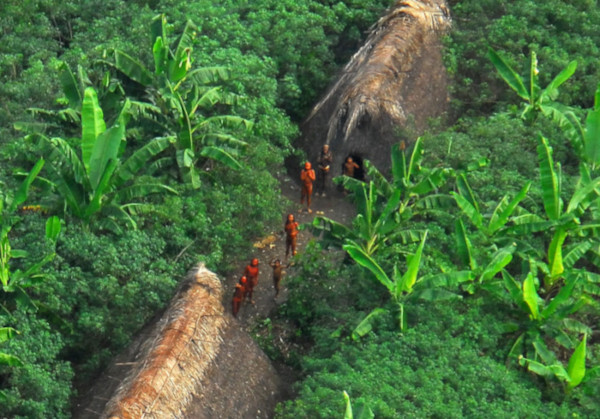
\includegraphics[width=0.95\linewidth]{images/Libro-img043.jpg}
  \begin{minipage}{\linewidth}
    \caption{Credits: Di Agência de Notícias do Acre: Gleilson Miranda / Governo do Acre -
\raggedright\url{https://www.flickr.com/photos/fotosdoacre/3793141477/,} CC BY 2.0,
\raggedright\url{https://commons.wikimedia.org/w/index.php?curid=18968640} }
  \end{minipage}
\end{wrapfigure}

Sono quei popoli indigeni che non hanno contatti con la civiltà moderna, secondo Survival International, le tribù
incontattate nel mondo sarebbero almeno 100. Nonostante il grado di conoscenza che abbiamo del nostro pianeta tutti gli
anni vengono scoperte nuove forme di vita vegetali e animali, ma ancora più incredibile è che ogni tanto vengono
scoperti nuovi gruppi di esseri umani. Nel 2009 in Brasile, dove si stima essere presente la maggior parte di questi
popoli, sono stati avvistati da un elicottero un nuovo gruppo di indigeni (immagine qui di fianco). 

La difficoltà di avere contatti con queste popolazioni è che spesso, quando avvengono contatti con noi occidentali
facciamo contrarre loro malattie e forme di influenza che non conoscono e di cui non hanno anticorpi e che possono
portare alla decimazione di queste comunità.

\begin{wrapfigure}{i}{9cm}
  \centering
  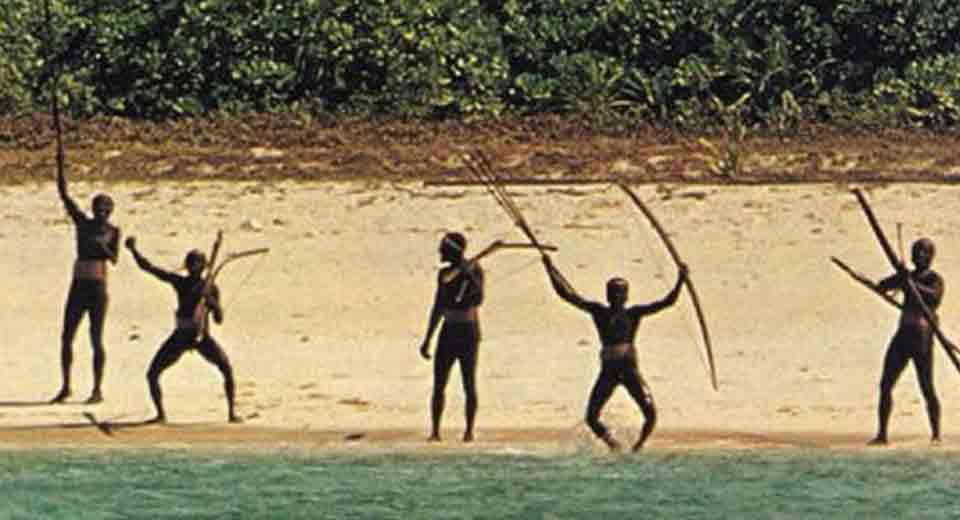
\includegraphics[width=0.95\linewidth]{images/Libro-img044.jpg}
  \begin{minipage}{\linewidth}
    \caption{Credits: Estratto di un filmato sulla tribù di north
sentinel che reagisce con arco e frecce agli estranei, Credit: Survival International}
  \end{minipage}
\end{wrapfigure}

Tra queste, la più isolata in assoluto è quella dell'Isola di North Sentinel nel golfo del Bengala.
Questa popolazione non conosce il remo per poter allontanarsi dall'isola e
l'India ha proibito di avvicinarsi in quanto, i numerosi tentativi di stabilire un contatto con
queste popolazioni si sono conclusi in modo violento da parte degli indigeni. Ci sono alcuni video risalenti agli anni
70 che potete trovare su internet del tentativo di avvicinarsi a questa comunità le quali hanno risposto scagliando
numerose frecce. Questa comunità è stata dichiarata da Survival International, la società più vulnerabile del pianeta,
in quanto una piccola epidemia potrebbe spazzare via i 50 abitanti (circa) di questo luogo.

\subsection{Paradismo}
Il Paradismo è un sistema politico simile al comunismo, ma senza proletariato. In un sistema paradista, i robot
sostituiscono la forza lavoro umana. Tutti i beni e i servizi (tra cui produzione e raccolta del cibo, consegna a
domicilio automatica, robot-chirurghi, ecc..) verranno nazionalizzati renderanno il denaro obsoleto, dal momento che
sarà tutto gratuito. In questo sistema i politici eletti lavoreranno mossi da un sincero desiderio di utilità verso
l'Umanità in quanto non godranno di benefici economici. Così, invece di lavorare unicamente per guadagnare denaro, gli
esseri umani potranno lavorare su ciò che amano: creare, studiare, ricerche, opere d'arte, musica, sviluppo
personale\endnote{\raggedright\url{https://it.paradism.org/page.php?8} }.

\subsection{Pedofilia}
Vivere con certezze su tutto, sicuramente ci da un ordine e serenità ma è un illusione. Uno degli scopi di questo libro
è proprio questo. Non avere certezze, mettere in discussione tutto e, vedere che quello che è vero per me magari non lo
è per te e viceversa. Però ci sono delle cose su cui possiamo dire tutti, all'unanimità, con certezza che sono giuste o
sbagliate no? Per esempio, i pedofili sono sbagliati! Su questo siamo tutti d'accordo e non ci piove! O forse no?
Discorso spinoso...

Ho trovato interessante questo
articolo\endnote{\raggedright\url{https://www.vice.com/it/article/aev5vj/un-pedofilo-si-rivolge-ai-suoi-detrattori} } dove viene
intervistato Todd Nickerson, 43 anni, vergine. Fa il grafico, vive solo in una roulotte e, per molto tempo è rimasto
chiuso nella sua camera, isolato, perché ha un segreto: è attratto dai bambini.

Nickerson è un pedofilo, prova pulsioni sessuali per i bambini a cui però non ha mai dato seguito, né lo farà mai in
futuro.

Secondo alcune stime i pedofili sono tra lo 0,5\% e il 2\% della popolazione, ma tra i reati di pedofilia tra il 40\% e
il 75\% non sono compiuti da pedofili. Queste persone, attratti da adulti, usano i bambini in sostituzione di un
partner sessuale adulto.

{\textquotedbl}Ci sono persone che sanno di avere pulsioni sessuali nei confronti dei bambini, e che per tutta la loro
vita non fanno niente, non scaricano pornografia infantile, non infrangono la legge,{\textquotedbl} dice James Cantor,
uno psicologo e studioso della sessualità.

I media così definiscono pedofili tutte le persone che commettono reati sessuali su minori alimentando questa
confusione.

Spesso alle spalle di adulti che sentenziamo come malvagi, anche al di fuori della pedofilia, troviamo storie di bambini
innocenti e senza colpe che hanno subito dei traumi. Anche Nickerson, racconta di essere stato molestato quando aveva
sette anni da un amico di famiglia, identificandosi in quella persona siccome era molto gentile e mostrava interesse
per lui. Nickerson si accorse di avere desideri diversi dagli altri quando aveva 13 anni, quindi, quando ancora era lui
stesso un bambino. I suoi coetaei dicevano di essere attratti dalle ragazzine più sviluppate mentre lui si accorse, a
casa dei nonni, quando arrivarono i vicini con la loro figlia di sette anni, di essere attratto dalle bambine non
ancora sviluppate. Da quel momento cercò di negare a se stesso di avere queste pulsioni, pregò perché Dio gli togliesse
questo fardello. Nickerson racconta che all'età di 18 anni si innamorò di una bambina di 5. {\textquotedbl}Si toglieva
i vestiti e correva per casa,{\textquotedbl} dice. {\textquotedbl}Quella bambina è stata l'unica nella mia vita che mi
ha messo davvero in tentazione.{\textquotedbl}

A quel punto Nickerson smise di fare il baby sitter, cambiò città, si impose di evitare i bambini e provò ad avere
relazioni con persone adulte, uscì con delle ragazze ma sentiva di non provare nessuna attrazione, capì che non sarebbe
mai successo, non avrebbe mai avuto una vita normale. In seguito arrivò la depressione, momenti di dolore e iniziò a
pensare al suicidio.

Nella ricerca di aiuto si iscrisse su Girlchat un forum per pedofili della fazione
{\textquotedbl}pro-contact{\textquotedbl}, dove si sostiene un cambio delle leggi sul consenso per legalizzare il sesso
con minorennim anche se, quest'ultimo punto non trovava approvazione da Nickerson. Poter parlare con altre persone fu
una grossa liberazione per lui, ma poco dopo, un gruppo di vigilanti, infiltratosi dentro questo forum ha raccolto
informazioni e foto di Nickerson che sono poi state rese pubbliche con volantini affissi nella sua città. Nickerson
perse così il lavoro e, anche a suo padre fu riservata la stessa sorte.

{\textquotedbl}Hanno letteralmente reso la mia vita più miserabile che potessero{\textquotedbl}.

Dopo essersi disiscritto da Girlchat diventò moderatore di Virtuous Pedophiles, un gruppo di supporto privato per
pedofili (1845 membri) che vogliono evitare di commettere crimini. Per quanto i vigilanti siano mossi da nobili motivi,
secondo \ Nickerson e la sua esperienza possono essere controproducenti alla battaglia contro le violenze sessuali sui
minori in quanto non sono regolamentati, come altre forze dell'ordine, con standard etici. I
vigilanti per trovare i pedofili online creano profili falsi di minorenni, con tanto di foto, dove con insistenza li
invitano ad incontrarsi. Come se uno volesse essere un buon marito ma venisse seguito sul luogo di lavoro e dentro
casa, siccome internet ormai è sempre con noi, dal una donna che rappresenta il massimo del suo desiderio sessuale,
oggi, domani, dopodomani, per sempre se necessario, fino a quando non arriva un momento di debolezza.

Anche secondo Cantor, stigmatizzare la pedofilia non fa altro che mettere in pericolo i bambini. Se la società pensa che
tu sia feccia anche se non hai mai commesso un crimine a lungo andare trovi poche motivazioni per continuare a
resistere. Una volta individuate queste persone sarebbe più producente farli ragionare su quello che stanno facendo,
farli parlare, offrirgli aiuto psicologico o farmacologico per la riduzione della libido rispetto alla gogna pubblica
che lo porterebbe alla depressione o al suicidio. Se un pedofilo viene trattato come un ladro o un assassino, lui si
comporterà esattamente allo stesso modo, cercando di compiere le loro azioni di nascosto. Sarebbe meglio invece che
venissero allo scoperto in modo che possano essere aiutati. La cosa che mi ha fatto riflettere è stata che lui non ha
scelto di diventare pedofilo, non ha scelto di essere abusato quand'era piccolo, però è successo e
ora dovrà faticare dieci volte tanto per sentirsi meglio rispetto a una persona “normale”. Purtroppo è così da sempre,
alcune persone casualmente, senza meriti o senza colpe, casualmente si trovano ad affrontare vite diverse, alcune più
semplici alcune più dure. Essere felici e accettati non è un nostro merito. Forse anche noi, se fossimo cresciuti un un
certo ambiente saremmo pedofili, ladri, assassini, ecc… Risulta quindi difficile giudicare una persona o sentirci
migliore di lei solo perché abbiamo avuto fortuna. Tutte le persone che non fanno del male agli altri meritano di
essere felici.

Immaginate di essere proiettati in un universo parallelo dov'è condannato il sesso eterosessuale.
Immaginate voi, per come siete, con i vostri desideri e le vostre passioni e che non potete più fare sesso, o che
dovete farlo di nascosto, solo dopo che sareste riusciti ad accettare che secondo gli altri avete un problema. Quando
vedete un bel ragazzo o una bella ragazza, dovete pensarci su due, tre, quattro, dieci volte prima di dichiararvi
perché potrebbe dirlo a tutti che vi potrebbero prendere in giro. Così è come vive un omosessuale che non ha nessuna
colpa di esserlo e che non ha mai molestato nessuno. Discorso simile può essere fatto per i pedofili, o qualsiasi altra
minoranza.

\subsection{Cannibali}
E i cannibali? Possiamo dire che questo è sicuramente sbagliato? Non nelle tribù indigene, ma quando un occidentale, un
europeo mangia un'altra persona? Sappiamo che il cannibalismo, in base alle mutilazioni ritrovate
su alcuni scheletri, avere origine già nel neolitico. Ne esistono di tre tipi, quello spirituale, dove alcune culture
indigene sacrificano corpi agli idei e assumendo la forza della loro vittima, quello legato alla sopravvivenza e infine
quello criminale che è spesso a sfondo sessuale. Avete capito bene, alcune persone trovano appagamento sessuale dal
mangiare altre persone e, come tutta la sessualità c'è un attivo e un passivo. Il passivo non
viene chiamato così perché viene costretto dall'attivo. Entrambi provano appagamento sessuale in
quella modalità. Alcune volte, parlando genericamente delle pratiche sessuali, si può provare piacere sia come attivo
che come passivo, per altre persone invece il piacere viene trovato solo nell'attività e per altri
nella passività. Molto famoso è stato il caso di Armin Meiwes. Sul web esistono siti di incontri per cannibali, dove si
possono inserire annunci dove si cercano persone che vogliono essere mangiate. Bernd-Juergen Brandes, un uomo distinto,
benestante di Berlino, rispose all'annuncio di Meiwes. Quest'ultimo gli
rispose inviandogli le foto della sua bocca dicendogli che con questi denti gli avrebbe staccato la lingua a morsi. 

\needspace{4cm}
\begin{wrapfigure}{i}{10.552cm}

\includegraphics[width=10.552cm,height=6.258cm]{images/Libro-img055.jpg}
\caption*{Armin Meiwes e Bernd-Juergen Brandes Credit: AP:Associated Press}
\end{wrapfigure}

Brandes prende il treno per andare da Meiwes, al suo arrivo si spoglia e inizia a bere un farmaco antinfluenzale che
dovrebbe provocare sonnolenza. L'adrenalina è tanta e Brandes resta sveglio. Così beve una
bottiglia di alcol seguite da 20 compresse di sonnifero ma ancora non riesce a tranquillizzarsi. A un certo punto la
vittima si decide e chiede di tagliarli il pene. Meiwes predispone una telecamera dove mostra la volontà di Brandes e
la sua consenzienza a essere mangiato come prova per un eventuale processo. In seguito Meiwes tagliò il pene di
Brandes, andrò in cucina dove iniziò a bollirlo insaporendolo con sale, aglio e pepe, poi lo divise in due e lo
consumarono assieme. La vittima perse molto sangue, gli venne preparato un bagno caldo e poi fatto sul letto dove restò
per dieci ore. All'alba Meiwes lo baciò, pregandolo di perdonarlo e, poi lo uccise. \ Quando
Meiwes venne scoperto raccontò che per la sua vittima fu stato bello, come se lo era immaginato, mentre per lui fu
strano. Sentì odio, gioia, furia, disgusto. Odio nei confronti di Brandes che l'ha portato a fare
questo e, odio nei confronti di se steso perché lo voleva fare. Raccontò anche del controverso rapporto con la madre,
molto autoritaria, austera, con manie di controllo. Quando compiette vent'anni, la madre applicò,
sulla camera del figlio, un cartello con scritto “stanza dei bambini”. Non aveva una vita sociale né sessuale e quando
provava a uscire con una ragazza la madre era sempre nei paraggi. Persino durante il periodo militare la madre andava a
trovarlo, mettendolo in imbarazzo di fronte ai suoi commilitoni. Un anno dopo la morte della madre mise il suo primo
annuncio.

La difesa, con le documentazioni video, voleva inquadrare il suo reato come “omicidio su commissione”, al pari
dell'eutanasia con una pena inferiore ai 5 anni di reclusione. Inoltre, aveva due testimoni.
Queste due persone risposero agli annunci di \ Meiwes in due momenti distinti, entrambi andarono a casa sua per essere
mangiati. Mentre Meiwes tracciava con un pennarello i segni dove praticare le incisioni per la macellazione i due
cambiarono idea e vennero liberati. \ Meiwes mangiava solo persone consenzienti. Secondo \ Meiwes, in base ai messaggi
che negli anni ha scambiato con altre persone ha stimato l'esistenza di almeno 800 cannibali in
Germania. Durante il processo si stabilì che Meiwes non era affetto da patologie psicologiche ma non si poteva
affermare lo stesso di \ Brandes così gli venne dato l'ergastolo. Chiaramente la salute mentale di
Brandes è l'elemento con il peso maggiore su questa bilancia. È comunque interessante, come
esercizio, proprio perchè ogni fibra del nostro corpo ci suggerisca essere una cosa sbagliata, ipotizzare, nel caso in
cui Brandes fosse stato consapevole della sua scelta, cosa possibile ma che non sapremo mai, comunque possibile come
caso ipotetico, cosa possiamo trovare di sbagliato in questo? Da un punto di vista il più distaccato e freddo
possibile, nessuno ha violato la libertà altrui, ed entrambi erano consenzienti.

In questo documentario\endnote{\raggedright\url{https://www.youtube.com/watch?v=GmJHfJlk9p8} } ho apprezzato molto
l'intervento di Umberto Galimberti: L'ombra è presente in ciascuno di noi
(tengo a sottolineare: in ciascuno di noi) come costitutiva della nostra psiche. Purtroppo noi veniamo da una cultura
cristiana. Dico purtroppo perché la cultura cristiana ha diviso radicalmente il bene e il male, mentre tutte le cose
sono sostanzialmente ambivalenti. Tutte le religione ipotizzano che Dio sia bene ma anche male. Il cristianesimo ha
operato questa divisione e che scontiamo con le figure della perfezione e della santità (alte aspettative e pressioni
sociali) rimuovendo il male. Tutto ciò che è rimosso, ce l'ha insegnato Freud, ritorna e, siccome
non è accolto dalla nostra parte razionale finisce con l'essere un rimosso violento.
l'ombra e il male sono violenti perché non accettati dall'Io.

\subsection{Modelli narrativi}
Tutte le storie che conosciamo, dalla letteratura, ai film, alle fiabe sono riconducibili a pochi modelli narrativi. 

Per Carlo Gozzi e Georges Polti sono 36. Questa classificazione è ancora oggi utilizzata nelle scuole di scrittura
creativa e in alcuni software di generazione di trame. Le trame sono: Supplica, Il salvataggio, Vendetta che insegue il
crimine, Vendetta per una persona cara per una persona cara, Braccato, Disgrazia improvvisa, Sacrificare qualcuno,
Riot, Un tentativo audace, Rapimento, Enigma, Realizzazione, Odio tra i propri cari, Rivalità tra i propri cari,
Aggiustatore accompagnato da omicidio, Follia, Negligenza mortale, Incesto involontario, L'omicidio involontario di una
persona cara, Abnegazione per amore dell'ideale, Sacrificio di sé per il bene dei propri cari, Vittima di una gioia
incommensurabile, Sacrificio ai propri cari in nome del dovere, Rivalità degli ineguali, Aggiustatore, Ama il crimine,
Il disonore di una persona cara, Amore che incontra ostacoli, Amore per il nemico, Ambizione, Combatti contro Dio,
Gelosia ingiustificata, Errore di giudizio, Rimorso, Ritrovato di recente, Perdita di persone care 


\bigskip

Secondo Christopher Booker sostiene che le trame possibili possono essere ricondotte a 7 modelli di base e, ognuno di
essi viene strutturato in 5 fasi: anticipazione, sogno, frustrazione, incubo e soluzione. Le trame invece sono:
sconfiggere il mostro, dalle stalle alle stelle, ricerca, viaggio e ritorno, commedia, tragedia, rinascita.

Sono 7 le trame anche secondo Jessamyn West, che le divide in: uomo contro se stesso, uomo contro la società, uomo
contro uomo, uomo contro natura, uomo contro destino, uomo contro Dio (o Sovrannaturale), uomo contro macchina.

Altri modelli riescono a raggruppare le trame in ancor meno categorie, forse troppo a mio avviso, perché non spiegano il
modo in cui si sviluppano le storie: il modello di Foster-Harris prevede tre tipologie: con lieto fine, senza lieto
fine, storie che vengono narrate partendo dalla fine. Secondo Ronald Tobias, esistono solo le trame del corpo e le
trame della mente. Per Gustav Freytag esiste solo il viaggio dell'eroe, dove vede un evento
scatenante, azioni crescenti, climax, azioni calanti,
epilogo\endnote{\raggedright\url{http://www.vittoriorenuzzi.it/storytelling-trame-possibili-modelli-narrativi/} }.

Affascinante è la tavola periodica dello storytelling inventata da Richard Harris, che potete trovare sia in
inglese\endnote{\raggedright\url{https://jamesharris.design/periodic/} } che in
italiano\endnote{\raggedright\url{https://www.webnauta.it/wordpress/tavola-periodica-dello-storytelling-in-italiano/} }.

\subsection{Quanto tempo perdiamo?}
Quanto tempo passiamo in una vita a fare certe operazioni?

Ho sempre fatto questi calcoli e sono contento non essere l'unico ad avere questa
malattia\endnote{\raggedright\url{https://www.focus.it/cultura/curiosita/le-statistiche-del-tempo-che-perdiamo} }

Per esempio ho fatto 5 anni il pendolare, tra treno e metro ci mettevo 2 ore a raggiungere il posto di lavoro e 2 ore a
tornare, questo voleva dire che passavo più di un mese, giorno e notte sui mezzi pubblici, ogni anno!


\bigskip

In una vita intera spendiamo il nostro tempo in:

\begin{itemize}
\item fare benzina: 25 giorni
\item allacciarsi le scarpe: 6 giorni
\item andare in ascensore: 50 giorni
\item scaldare nel microonde: 9 giorni
\item tagliarsi le unghie: 13 giorni
\item riempire bicchieri: 9 giorni
\item aspettare il verde: (in auto) 38 giorni
\item aspettare il verde: (a piedi) 69 giorni
\item dipingersi le unghie: 13 giorni
\item farsi la barba: 76 giorni
\item allacciare i bottoni: 3 giorni
\item lavarsi i denti: 106 giorni
\item masticare: 140 giorni
\item fare il caffè: 35 giorni
\item lavarsi: 177 giorni
\end{itemize}

\bigskip

\subsection{Altre curiosità}

\bigskip

\begin{itemize}
\item Si può resistere da uno a due mesi senza mangiare (se si beve l'acqua).
\item Suoni di 185 - 200 decibel possono uccidere l'uomo. Il suono più forte mai udito
dall'uomo, o almeno misurato, fu l'eruzione del 1883 del Krakatoa (Indonesia) che distrusse i due
terzi dell'isola. Gli effetti, soprattutto climatici, si sentirono in tutto il pianeta per parecchi anni. Il fumo del
vulcano salì fino a 30 chilometri di altezza e si verificò un gigantesco tsunami, la cui onda più alta misurava 30
metri. Il rumore dell'esplosione è stato misurato a 172 decibel alla distanza di 160 km e fu udito
fino in Madagascar.
\item Possiamo resistere circa 3-4 minuti senza ossigeno, le prime cellule a morire sono quelle cerebrali. Se andiamo in
ipotermia perl, il corpo abbassa molto il metabolismo e si può resistere parecchi minuti in più.
\item Possiamo resistere 10 giorni senza dormire.
\item E 10 giorni senza acqua.
\item Nel deserto dell'Australia ogni 10 anni circa, grazie ai monsoni si forma il Lago Eyre. Tanti pellicani, che
popolano il lago, arrivano da centinaia di km, dalle coste australiane. Molti di loro lo vedranno soltanto una volta
nella vita. Come sappiano della sua esistenza e di come raggiungerlo resta un mistero. 
\item Il cervello lavora meglio sotto i venti gradi di temperatura
\end{itemize}